\section{Introduction}
\label{sec:intro}

Understanding animals' verbal expressions is an interesting interdisciplinary scientific challenge, 
in particular pet dogs, who are closely integrated with humans. 
Previous research endeavors to comprehend dog barking sounds for a number of reasons, such as for a better understanding of animal biological evolution\cite{pongracz2017modeling}, applying their language to information technology, or just curiosity about dogs' intention when they bark~\cite{pongracz2011children,dogbark_1}. However, this task is challenging not only due to the unknown acoustic pattern of dogs but also the lack of a suitable and high-quality dataset.

Previous researchers have demonstrated that dog's barking sound indeed reflects their individual characteristics~\cite{pongracz2010barking,larranaga2015comparing}, emotional expression~\cite{thorndike2017animal,hantke2018my,paladini2020bark} and understanding of outside world~\cite{larranaga2015comparing, molnar2008classification}. However, despite the fact that dogs are human's closest friends, little research has looked into the influence on dogs' communication arising from their interaction with human hosts. Although there are many communication methods of dogs, we pay attention to their sounds, which serve as one of the most important communication  channels~\cite{siniscalchi2018communication}. In our work, we hypothesize that a dog's acoustic characteristics may be correlated with such interaction, particularly the host's language. To verify that, we explore the barking difference of a particular dog breed (Shiba Inu) from two different host language environments (English vs. Japanese)~(\figref{fig:intropic}). Shiba Inu dogs are chosen as the subject of this study because Shiba Inus are very popular among dog owners and there is an abundance of their audio/video resources available online.  Moreover, we choose to work on dogs in English and Japanese language environments because these two widely-spoken languages have very different phonetic systems, and at the same time, Shiba Inu dogs are very popular in Japanese and English-speaking households (i.e., in Japan and in the US).

\begin{figure}[th]
	\centering
	\scalebox{0.24}{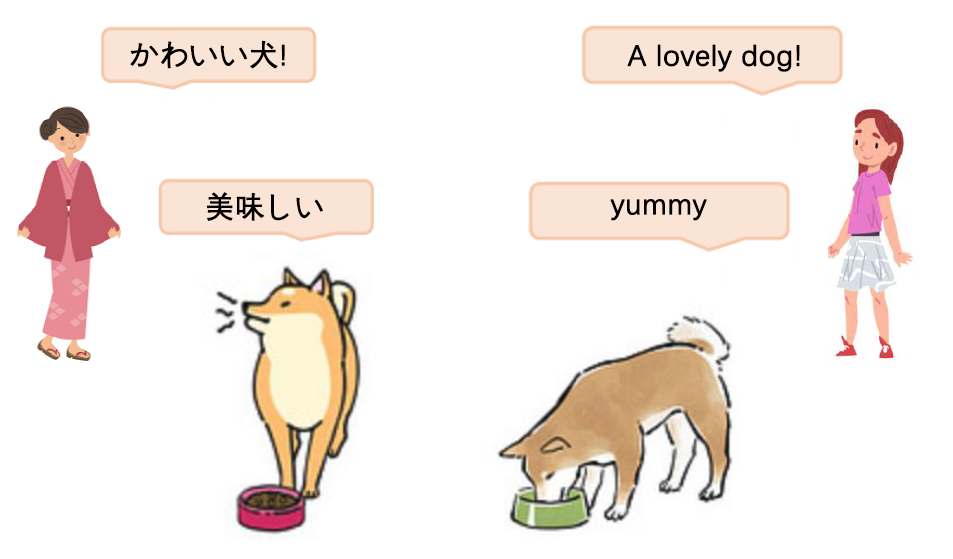
\includegraphics{images/intropic_big_add11.png}}
	\caption{%\KZ{remove the scene tags from the pic.} 
Our hypothesis is that a dog's barking 
may be accousticly correlated with its host language, 
so that a ``Japanese'' dog should bark differently than an ``American''
dog under the same context such as ``eating on the lawn''.}
	\Description {introducing scenario: two shiba inu dogs interact with its hosts in different Japanese and English environment.}
\label{fig:intropic}
\end{figure}

We verify the above hypothesis in two steps. 
First, we conduct classification experiments to investigate the possible
existence of interesting acoustic properties that distinguish dog barks from one language environment to the other. The classification experiment is performed on pairs of Japanese and English dog barking clips under the same \textit{context} which is composed of the \textit{scene category}, \textit{location}, and \textit{activity} of the barks so as to exclude  
these confounding non-linguistic factors, which may influence how dogs bark. 

In step two, to discover the most prominent factors that distinguish dog barks by their language environment, we perform an importance analysis of different factors using Shapley values. A similar analysis is also performed on host languages, to study the acoustic difference between English and Japanese. Moreover, we compute the Pearson correlation between dog barks and their host speech. 
The fact that several most important acoustic characteristics differentiating dogs have 
substantial correlations with those of their host language (i.e., English or Japanese) supports 
our hypothesis that the domestic dog barking does share a few acoustic similarities with its 
host language. It is possible that the host language environment has an influence over 
the dog's barking. 

Previously, the datasets for the barks of dogs are mostly collected by raising a dog and recording 
the sounds~\cite{ide2021rescue, ehsani2018let, molnar2008classification, hantke2018my}. As this method costs a lot and there is no public-released Shiba Inu barks dataset, 
we derive a pipeline to obtain and extract the barks from social media. Moreover, 
the context information is tagged along the bark to help us eliminate the confounding factors 
in our experiments. To construct the dataset ``EJShibaVoice'', we develop 
a framework that crawls Shiba Inu audio clips from both English and 
Japanese-speaking host families, extracts the barking sound clips, 
segments the clips into contiguous singular barks, and tags them with contextual information. 


Our main contributions are summarized as follows:

\begin{itemize}
	\item We define a new task to uncover the human linguistic influence 
on the vocal expression (barks) of domestic Shiba Inu dogs, 
which can inspire further research on animal 
languages.~(\secref{sec:assumption})
	\item We construct a Shiba Inu barks dataset \textbf{EJShibaVoice} with a pipeline containing clean audio clips produced by dogs from two different language environments: English and Japanese, including dogs' host speech clips. 
The barks and speech data undergo a systematic pipeline, which extracts clean barks and 
the corresponding host speech from the social media videos.~(\secref{sec:assumption})
	\item We discover prominent acoustic differences between dogs 
from different language environments: 
	Shiba Inus barks from English-speaking households have a \textit{lower frequency}, 
while those from Japanese environments have \textit{faster speed}, 
which correlates with these two human languages, respectively.~(\secref{sec:main})%by testing several kinds of audio features on our pairwise dataset.
\end{itemize}
